\chapter{Exercises}
\label{ch:exercises}

\section{The basics}
\label{sec:ex-basics}

\begin{enumerate}
\item Plot the sine and cosine functions from 0 to 2$\pi$.
  
\item Write a function to plot an ellipse:
  \[
  \begin{cases}
    x = a\cos(\alpha)\cos(\beta) - b\sin(\alpha)\sin(\beta)\\
    y = a\sin(\alpha)\cos(\beta) + b\cos(\alpha)\sin(\beta)
  \end{cases}
  \mbox{where~}0 \leq \beta \leq 2\pi
  \]

  \noindent and $\alpha$ is the rotation angle of the ellipse.
  
\item Write a function that takes two numbers as input and tells the
  user whether these are multiples of each other or not.

\item Write a function to print the following number triangle:

  1\\
  2 2\\
  3 3 3\\
  4 4 4 4\\
  5 5 5 5 5\\
  $\vdots$
  
  down to any value $n$
  
\end{enumerate}

\section{Plotting data}
\label{sec:ex-plotting}

\begin{enumerate}
  
\item Using \texttt{geostats}' \texttt{countQuakes} function
  (section~\ref{sec:R-basics}.\ref{it:geostats}), plot the declustered
  earthquakes of magnitude 4.5 and greater from 2000 to 2016 as a bar
  plot, and as a histogram.

\item\label{it:AB} Generate two samples ($A$ and $B$, say) of 100
  random numbers between 0 and 1; calculate the ratios $A/B$ and
  $B/A$; and create a ${2}\times{2}$ figure with KDEs and rug plots of
  $A/B$, $B/A$, $\ln(A/B)$ and $\ln(B/A)$.
  
\item\label{it:randxy} Create a bivariate ($x$, $y$) dataset of 1000
  random uniform numbers where $-1\leq{x}\leq{+1}$ and
  $2\leq{y}\leq{22}$. Construct a 2-dimensional KDE for these data.
  
\item Plot the ECDFs of the $x$ and $y$ values of the previous
  exercise. What fraction of the $x$-values is less than 0?  What
  fraction of the $y$-values is less than 7? And less than 17?

\end{enumerate}

\section{Summary statistics}
\label{sec:ex-summary-statistics}

\begin{enumerate}
  
\item Calculate the means and variances of the Anscombe quartet, and
  store them in a ${2}\times{8}$ matrix.

\item Generate $n=10$ random numbers between 0 and 1. Calculate their
  mean. Repeat 100 times and store the mean values in a 100-element
  vector. Compute the mean and standard deviation of this vector.
  Repeat for $n=100, 1000$ and $10000$.

\item Generate 1000 random numbers between 0 and 200. Count the number
  of values that are less than 1. Repeat 500 times to fill a vector of
  counts. Compute the mean and variance of this vector.
  
\item Generate two samples ($A$ and $B$) of 100 random numbers between
  0 and 1, and calculate their logratio $\ln(A/B)$. Repeat 10 times
  and visualise the results as a box plot.

\end{enumerate}

\section{Probability}
\label{sec:ex-probability}

\begin{enumerate}
  
\item The International Geo Sample Number (IGSN) is an alphanumeric
  code that is used to identify geological rock specimens in the
  scientific literature. It consists of one to five letters to
  identify the owner of the sample, followed by four characters
  (letters or numbers) to identify the sample itself. Examples are
  PVERM1234 and UCL001B. How many samples can each owner register? How
  many possible IGSNs are there in total?

\item 20 students are taking part in a mapping exercise. How many ways
  are there to divide them into 4 distinct groups of 5?
  
\item A thoroughly mixed conglomerate contains 30\% andesite clasts,
  20\% basalt clasts, and 50\% carbonate clasts. How many randomly
  selected clasts do we need to pick to be 95\% certain that we have
  collected at least one clast of each lithology?

\item 95\% of iron ore deposits are characterised by magnetic
  anomalies, and so are 98\% of chromium deposits and 1\% of other
  rocks.  0.1\% of all rocks contain iron ore, and 0.05\% of rocks
  contain chromium ore. Suppose that we have found a magnetic anomaly.
  What is the probability that this is caused by an ore deposit?

\end{enumerate}
  
\section{The binomial distribution}
\label{sec:ex-binomial}

\begin{enumerate}
  
\item In palynology, the ratio of arboreal to non-arboreal pollen is
  widely used as an index of landscape openness. This ratio is
  estimated by counting a representative number of randomly selected
  pollen from a soil sample.  Suppose that we have counted 20 pollen
  and counted the number of arboreal or non-arboreal species among
  them. Further suppose that the true arboreal/non-arboreal pollen
  ratio in the soil is 4. What is probability that the
  arboreal/non-arboreal ratio of the 20 \emph{counts} is 9 or greater?

\item We believe that 50\% of all dinosaur fossils are female (and
  50\% are male). A bone bed contains 50 dinosaur fossils among which
  32 are female (and 18 are male). Do we have enough evidence to prove
  that the proportion of males and females is different?  Do our data
  support the notion that females are more common than males?

\item Draw 50 random numbers from a binomial distribution with $p=0.2$
  and $n=100$. For each of these values, perform a two-sided test
  against the null hypothesis that $p=0.2$. Do all the values pass the
  test?

\item Given $A=12$ arboreal pollen and $N=8$ non-arboreal pollen,
  compute a 95\% confidence interval for the $A/N$-ratio of the soil.


\end{enumerate}

\section{The Poisson distribution}
\label{sec:ex-poisson}

\begin{enumerate}
  
\item On average a magnitude $\geq{9}$ earthquake occurs once every
  13.5 years. What is the probability that two such earthquakes will
  happen next year?  What is the probability that none will happen in
  the next century?

\item The fission track method is a geochronological technique that is
  based on the spontaneous fission of \textsuperscript{238}U in
  accessory minerals such as apatite. Spontaneous fission occurs with
  a probability of $8.46\times{10}^{-17}$ per atom of
  \textsuperscript{238}U per year. This is known as the decay
  constant. Suppose that a 1~million year old apatite crystal contains
  1~pmol of \textsuperscript{238}U ($=6.022\times{10}^{11}$
  atoms). What is the probability that it contains 50 or fewer fission
  tracks? What is the probability that it contains 41 to 60 tracks?
  
\item The Orange River in South Africa is famous for its alluvial
  diamonds. In order for mining operations to be profitable, placer
  deposits must contain at least 2 diamonds per tonne.  A diamond
  mining company has sieved 10 tonnes of sand and found 12
  diamonds. Assuming that the diamonds are randomly distributed in the
  sand, should the company cease operations? Or would it be premature
  to do so and should they acquire some more data first?

\item At another site, a preliminary mining survey has yielded 30
  diamonds in 10 tonnes. Construct a 95\% confidence interval for the
  diamond yield in this deposit.
  
\end{enumerate}

\section{The normal distribution}
\label{sec:ex-gauss}

\begin{enumerate}

\item Generate 100 random numbers from a Poisson distribution with
  $\lambda=1.2$ and take their sum. Repeat this 200 times and plot the
  results as a histogram. Calculate the mean and the standard
  deviation of this synthetic dataset. What percentage of the values
  falls within two standard deviations from the mean?
  
\item The 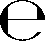
\includegraphics[height=0.7em]{../figures/e.pdf}-symbol on
  packaging guarantees consumers that they receive at least the amount
  of product that they paid for. For example,
  0.75\,L\,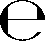
\includegraphics[height=0.7em]{../figures/e.pdf} means that
  at most 1.5\% of the containers with this label are allowed to
  contain less that 0.75\,L of fluid.  Suppose that the amount of wine
  that is dispensed by a bottle filling machine follows a normal
  distribution with a standard deviation of 2\,ml.  On average, by how
  much do we have to overfill the bottles to ensure that our wine
  receives the 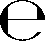
\includegraphics[height=0.7em]{../figures/e.pdf}-label?
  Work out the solution by hand using Table~\ref{tab:normal}.
  
\item The height of men follows a normal distribution with a mean of
  175\,cm and a standard deviation of 7.7\,cm. The height of women
  follows a normal distribution with a mean of 160\,cm and the same
  standard deviation. Using Table~\ref{tab:normal}, determine the
  approximate percentage of men who are shorter than the tallest 10\%
  of women.

\item Using a normal approximation to the Poisson distribution,
  calculate the probability of $k<{62}$ when $\lambda=64$.
  
\item Consider two bivariate normal distributions with mean vectors
  $\mu_X$ and $\mu_Y$, and covariance matrices $\Sigma_X$ and
  $\Sigma_Y$, respectively:
  \[
  \mu_X =
  \left[
    \begin{array}{c}
      1\\
      2
    \end{array}
    \right]\mbox{,~}
  \Sigma_X =
  \left[
    \begin{array}{cc}
      1 & -1\\
      -1 & 3
    \end{array}
    \right]\mbox{,~}
  \mu_Y =
  \left[
    \begin{array}{c}
      3\\
      4
    \end{array}
    \right]\mbox{~and~}
  \Sigma_Y =
  \left[
    \begin{array}{cc}
      2 & 2\\
      2 & 7
    \end{array}
    \right]  
  \]

  Which outcome is most likely:
  \[
  X =
  \left[
    \begin{array}{c}
      2\\
      1
    \end{array}
    \right]\mbox{~or~}
  Y =
  \left[
    \begin{array}{c}
      5\\
      7
    \end{array}
    \right]\mbox{?}
  \]
  
\end{enumerate}

\section{Error propagation}
\label{sec:ex-errorprop}

In the following questions, the uncertainties are assumed to be
independent (i.e. covariances are zero).

\begin{enumerate}
  
\item The height difference between Ordnance Survey benchmark A and a
  second point B is $25\pm0.25$~m, and the height difference between B
  and a third point C is $50\pm0.5$~m. Calculate the height difference
  between A and C and propagate its uncertainty.
  
\item Consider the following two rock specimens:

\begin{tabular}{ccccc}
specimen & mass (g) & $\sigma$(mass) & volume (cm$^3$) & $\sigma$(volume) \\
\hline 
A & 105 & 2 & 36 & 0.15\\
B & 30 & 2.5 & 10 & 0.4
\end{tabular}

\begin{enumerate}
\item Compute the densities of rocks A and B.
\item Propagate their respective uncertainties.
\item Construct approximate 95\% confidence intervals for the two densities.
\item Is there a significant difference in density between samples A and B?
\end{enumerate}

\item Sand may contain a variety of minerals with different densities.
  For example, zircon has a density of
  $\rho_z=4.85\pm0.10$~g/cm\textsuperscript{3} (1$\sigma$), whereas
  quartz has a density of $\rho_q=2.65\pm0.05$~g/cm\textsuperscript{3}
  (1$\sigma$).  The settling velocity of sand grains in water depends
  on two factors: density and grain size. Dense grains settle more
  quickly than light ones, and large grains settle more quickly than
  small ones. When a balance is reached between these two factors,
  small zircons settle at the same rate as large quartz grains. This
  results in a \emph{size shift} ($SS$)\footnote{$SS \equiv
    \log_2(D_z/D_q)$ where $D_z$ = diameter of zircon grains and $D_q$
    = diameter of quartz grains.} between zircon and quartz in beach
  and river sands, which can be predicted from their respective
  densities:
\[
SS = \frac{1}{0.69}\ln\left(\frac{\rho_z-1}{\rho_q-1}\right)
\]

Calculate $SS$ and propagate its uncertainty.

\item We measured the following \textsuperscript{40}K and
  \textsuperscript{40}Ar concentrations:
  \begin{center}
    \begin{tabular}{c|cccccc}
      \textsuperscript{40}K ($\times$10$^{-10}$ mol/g) & 2,093 & 2,105 & 2,055 & 2,099 & 2,030 & ~ \\
      \textsuperscript{40}Ar ($\times$10$^{-10}$ mol/g) & 6.015 & 6.010 & 6.030 & 6.005 & 6.020 & 6.018 
    \end{tabular}
  \end{center}
\begin{enumerate}
\item Calculate the mean $^{40}$K and $^{40}$Ar concentrations.
\item Calculate the standard error of these means.
\item Estimate the $^{40}$Ar/$^{40}$K-ratio and its standard error.
\item The age equation for the $^{40}$K-$^{40}$Ar method is as follows:
\[
t = \frac{1}{\lambda} \ln\left[ 1 + \frac{\lambda}{\lambda_e}
  \left(\frac{^{40}Ar }{^{40}K}\right) \right]
\]

with $\lambda$ = 5.543 $\times$ 10$^{-4}$ Myr$^{-1}$ and
$\lambda/\lambda_e$ = 9.3284.  Calculate the age and its standard error.
\end{enumerate}

\end{enumerate}

\section{Comparing distributions}
\label{sec:ex-comparingdistributions}

\begin{enumerate}

\item\label{it:wine-t} We have measured the contents of five randomly
  selected bottles of wine:
  \[
  750.1, 750.4, 749.9, 750.3, 750.3
  \]

  \begin{enumerate}
    \item\label{it:one-sided} Can we conclude, at a 95\% confidence
      level, that the mean volume exceeds 750\,ml?
    \item\label{it:two-sided} Can we conclude that the mean volume is
      \emph{different} than 750\,ml?
    \item Compute a 95\% confidence interval for the mean volume of
      the wine bottles.
  \end{enumerate}

  Work the solutions out by hand using Table~\ref{tab:t} and check the
  results with \texttt{R}.

\item \texttt{geostats} contains a dataset with foraminifera counts
  for two surface sediments (A and B) from the Atlantic Ocean:

\begin{console}
> data(forams,package='geostats')
> forams
  uvula scitula quinqueloba pachyderma incompta glutinata bulloides
A     9       1          13         15       16        10        10
B    20      15          35         30       40        20        18
\end{console}

Is there sufficient evidence that the two samples represent different
ecosystems, i.e. that the proportions of the different species in both
samples is significantly different?
  
\item Using Table~\ref{tab:chi2}, test if the following histogram is
  consistent with a uniform distribution:
  
    \begin{tabular}{c|ccccc}
      count & 20 & 28 & 16 & 12 & 24 \\
      bin  & 0-20 & 20-40 & 40-60 & 60-80 & 80-100
    \end{tabular}

\item A gemologist has ranked 15 diamonds in order of increasing
  quality. The diamonds belong to two different categories: synthetic
  (`S') and natural (`N'):

    \begin{tabular}{@{}r@{~~}|r@{~~}r@{~~}r@{~~}r@{~~}r@{~~}r@{~~}r@{~~}r@{~~}r@{~~}r@{~~}r@{~~}r@{~~}r@{~~}r@{~~}r@{}}
      rank & 1 & 2 & 3 & 4 & 5 & 6 & 7 & 8 & 9 & 10 & 11 & 12 & 13 & 14 & 15 \\ \hline
      variety & N & S & N & N & S & S & S & N & N & N & N & S & S & S & S
    \end{tabular}

  Using Table~\ref{tab:wilcox}, is there a statistically significant
  difference in quality between the two diamond varieties at a 95\%
  confidence level?
    
\item Compare the following two samples, first with a t-test, then
  with a Wilcoxon test:

    \begin{tabular}{c|ccccccc}
      A & 0 & 2 & 4 & 6 & 8 & & \\
      B & 3 & 5 & 7 & 9 & 11 & 13 & 15
    \end{tabular}

  Which of the two tests is more powerful?
  
\item The \texttt{DZ} dataset in the \texttt{geostats} package
  contains a list of 15 detrital zircon U--Pb age
  distributions. Calculate the Kolmogorov-Smirnov statistic for all
  possible pairs of samples. Which two samples are the most similar?
  Which are the least similar? Show the resulting two pairs as two Q-Q
  plots.
  
\end{enumerate}

\section{Regression}
\label{sec:ex-regression}

\begin{enumerate}
\item \texttt{trees} is one of \texttt{R}'s built-in datasets. Have a
  look at it by typing \texttt{plot(trees)} at the command prompt. Now
  calculate the correlation coefficients of all possible combinations
  of variables. Which variables have the strongest correlation?
  Determine the corresponding slope and intercept.

\item \texttt{geostats} contains a dataset called \texttt{worldpop},
  which tallies the world's population from 1750 until 2014.  From
  1960 onwards, the world population has been growing at a linear
  rate. Fit a straight line through these values and extrapolate it to
  today. Then compare your prediction with the value reported on
  \href{https://www.worldometers.info}{\tt
    https://www.worldometers.info}.

\item Let $x$, $y$ and $z$ be three independent normally distributed
  sets of $n=100$ measurements with coefficients of variation
  $\sigma_x/\mu_x=0.05$, $\sigma_y/\mu_y=0.01$ and
  $\sigma_z/\mu_z=0.1$, respectively.  Form two new variables by
  taking the ratios $X=x/z$ and $Y=y/z$. What is the expected null
  correlation for $X$ and $Y$? Compare with the actual value.

\item Consider the following three samples:
\begin{center}
\begin{tabular}{cccccc}
  $i$ & $x$ & $s[x]$ & $y$ & $s[y]$ & $cov[x_i,y_i]$ \\
  \hline
  1 & 10 & 1 & 20 & 1 & 0.9 \\
  2 & 20 & 1 & 30 & 1 & 0.9 \\
  3 & 28 & 1 & 42 & 1 & -0.9
\end{tabular}
\end{center}

Fit a straight line through the ($x_i, y_i$)-data, first ignoring the
uncertainties ($s[x_i]$, $s[y_i]$, $cov[x_i,y_i]$), and then using
error weighted regression.

\end{enumerate}

\section{Fractals and chaos}
\label{sec:ex-fractals}

\begin{enumerate}
  
\item Plot the size-frequency distribution of North American rivers
  using \texttt{R}'s built-in \texttt{rivers} dataset.

\item Use the \texttt{boxcount} function in \texttt{geostats} to count
  how many $4\times{4}$ boxes are needed to cover all the fractures in
  \texttt{geostats}' \texttt{fractures} dataset. How many $8\times{8}$
  boxes are needed? Compute the fractal dimension of the fracture
  pattern.
  
\item Using the last 50 years of the \texttt{geostats}'
  \texttt{declustered} dataset, estimate the chance of observing at
  least one magnitude $\geq$6 earthquake in the western United States
  next year. Hint: use a combination of fractal and Poisson
  distributions.

\item Use \texttt{geostats}' \texttt{pendulum} function to repeat the
  pendulum experiment of Section~\ref{sec:chaos}. Try different
  initial positions, velocities, numbers of magnets etc. See
  \texttt{?pendulum} for details.
  
\end{enumerate}

\section{Unsupervised learning}
\label{sec:ex-unsupervised}

\begin{enumerate}
  
\item Visualise \texttt{R}'s built-in \texttt{iris} dataset as a PCA
  biplot and interpret the results. Hint: remove the \texttt{Species}
  column from the \texttt{iris} data to get a matrix of
  four-dimensional data
  (Section~\ref{sec:R-unsupervised}.\ref{it:R-kmeans}).
  
\item Analyse the same \texttt{iris} data by MDS. Check if the results
  are consistent with the output of the previous exercise.

\item\label{it:ex-withinss} The \texttt{kmeans} function of
  Section~\ref{sec:R-unsupervised}.\ref{it:R-kmeans} returns a
  9-element list. This list includes an item called \texttt{withinss},
  which contains the sum of squared distances of all the items in each
  cluster to their respective centres, and another item called
  \texttt{tot.withinss}, which contains the sum of the
  \texttt{withinss} values. Plot the value of \texttt{tot.withinss}
  against the number of clusters ($k$) for the \texttt{iris} dataset,
  for $1\leq{k}\leq{10}$. The `elbow' in this curve marks the optimal
  number of clusters.

\item Use the \texttt{ksdist} function of the \texttt{geostats}
  package to create a distance matrix of Kolmogorov-Smirnov statistics
  for the \texttt{DZ} dataset. Then use the output of this function to
  build a hierarchical clustering tree for those detrital zircon U--Pb
  ages.  Are the results consistent with the MDS configuration of
  Figure~\ref{fig:DZmds}?
  
\end{enumerate}
  
\section{Supervised learning}
\label{sec:ex-supervised}

\begin{enumerate}
\item\label{it:LDA-training} The \texttt{geostats} package includes a
  dataset called \texttt{training}, which contains the
  SiO\textsubscript{2}, TiO\textsubscript{2},
  Al\textsubscript{2}O\textsubscript{3}, CaO, MgO, MnO,
  K\textsubscript{2}O and Na\textsubscript{2}O concentrations (in
  wt\%) of 227 island arc basalts (IAB), 221 mid oceanic ridge basalts
  (MORB), and 198 ocean island basalts (OIB). Build an LDA model for
  the data. What is the misclassification rate of the data?
  
\item\label{it:LDA-test} The \texttt{geostats} package also contains a
  second dataset of IAB, MORB and OIB compositions called
  \texttt{test}. Classify these data using the LDA model obtained
  under question~\ref{it:LDA-training}. What is the misclassification
  rate?  Compare this to the misclassification rate of the
  \texttt{training} data.

\item\label{it:rpart-training} Build a decision tree for the
  \texttt{training} data. What is the misclassification rate of the
  optimal tree?

\item\label{it:rpart-test} Analyse the \texttt{test} data with the
  decision tree of question~\ref{it:rpart-training}. How does its
  misclassification rate compare to that of the \texttt{training}
  data? And to the LDA analysis of questions~\ref{it:LDA-training} and
  \ref{it:LDA-test}?
  
\end{enumerate}
  
\section{Compositional data}
\label{sec:ex-compositional}

\begin{enumerate}

\item \texttt{mtcars} is one of \texttt{R}'s built-in datasets. It
  contains a table with the fuel consumption and 10 aspects of
  automobile design and performance for 32 automobiles features in a
  1974 edition of `Motor Trend' magazine.
  \begin{enumerate}
    \item\label{it:mpg1} Calculate the average fuel consumption of
      these 32 vehicles --which are listed in miles per gallon-- using
      the arithmetic mean.
    \item\label{it:mpg2} Convert the data to European units, namely
      litres per 100km. $x$ miles/gallon $= y$ litres/100km,
      where:
      \[
      y = \frac{235.21}{x}
      \]
    \item\label{it:mpg3} Calculate the arithmetic mean fuel
      consumption in litres/100km.
    \item\label{it:mpg4} Convert the arithmetic mean number of mpg
      (from step~\ref{it:mpg1}) to units of litres/100km.  How does
      the resulting value compare with that obtained from
      step~\ref{it:mpg3}?
    \item\label{it:mpg5} Compute the geometric mean fuel consumption
      in mpg and litres/100km. Then convert the units of these mean
      values and compare with the result observed under
      step~\ref{it:mpg4}.
  \end{enumerate}

\item Load \texttt{geostats}' \texttt{test} data into memory and plot
  the CaO--K\textsubscript{2}O--Na\textsubscript{2}O
  \textbf{subcomposition} on a ternary diagram. Add the arithmetic and
  logratio mean compositions to the plot. Experiment with the
  arguments to the \texttt{ternary} function to make the plot look as
  clear as possible.

\item Perform compositional PCA on the \texttt{test} data and
  interpret the results on a biplot. Use the optional \texttt{col}
  argument of the \texttt{biplot} function to enhance the figure.
  
\item Repeat the LDA exercise of
  Sections~\ref{sec:ex-supervised}.\ref{it:LDA-training} and
  \ref{it:LDA-test}, but using a logratio transformation. How does the
  transformation affect the misclassification rates?
  
\end{enumerate}

\section{Directional data}
\label{sec:ex-directional}

\begin{enumerate}

\item Consider the following two sets of compass bearings:

  \begin{tabular}{c|ccccc}
    $A$ & 50 & 55 & 40 & 60 & 45 \\
    $B$ & 350 & 10 & 5 & 358 & 
  \end{tabular}

  What is the difference of the vector means for $A$ and $B$?

\item The \texttt{earthquakes} dataset in the \texttt{geostats}
  package contains two columns with the longitude and latitude of
  20,000 earthquakes.  Extract the events that took place between
  longitudes $-90^\circ$W and +$90^\circ$E and plot them on a Schmidt
  stereonet.

\item Consider the following two sets of fault measurements:

  \begin{tabular}{c|cccc|ccccc}
    ~ & \multicolumn{4}{c|}{1\textsuperscript{th} fault} &
        \multicolumn{5}{c}{2\textsuperscript{nd} fault} \\ \hline
    strike & 200 & 195 & 210 & 205 & 20 & 25 & 18 & 17 & 16 \\
    dip    & 70  & 68  & 71  & 67 & 10 & 12 & 9  & 14 & 11
  \end{tabular}

  Plot the two sets of faults on a Wulff net and calculate the
  difference of their mean strike and dip.

\item Which of \texttt{geostats}' built-in datasets is more tightly
  clustered: \texttt{palaeomag} or \texttt{fault}?
  
\end{enumerate}

\section{Spatial data}
\label{sec:ex-spatial}

\begin{enumerate}

\item\label{it:hillsemivariogram} The \texttt{geostats} package
  contains a dataset called \texttt{hills}, which tabulates 250
  topographic measurements for a synthetic landscape comprised of
  three bivariate normal `hills'. Fit an exponential, Gaussian and
  spherical model to the semivariogram. Subjectively assess which
  model fits the empirical semivariogram best.

\item Using the semivariogram model obtained under
  question~\ref{it:hillsemivariogram}, estimate the elevation at
  position $\{x=0,y=0\}$, and its standard error.

\item Create a contour plot of the \texttt{hills} dataset.
  
\item Using the Meuse data, create a contour map of the difference
  between kriging models using a spherical and exponential
  semivariogram model.

\end{enumerate}
